\documentclass{article}

\usepackage{hyperref}
\usepackage{titlesec}
\usepackage{titling}
\usepackage[margin=0.2in]{geometry}
\usepackage{graphicx}
\usepackage{multicol}
\titleformat{\section}
{\large\uppercase}
{}
{0em}
%{}[\titlerule]
{}
%[runin]
\titleformat{\subsection}
{\bfseries}
{}
{1em}
{}[]

\renewcommand{\maketitle}{
    \begin{flushleft}        
        {\huge\rmfamily
        \theauthor}\newline
        \vspace{0.1em}
        \textit{Mail: sahilsainisalaria@gmail.com }  \newline  
        \textit{ Github: github.com/Sahil1515 }  \newline 
        \textit{ Contact: +91 9682663655 }  \newline 
        \textit{ Address: Jammu, Jammu \& Kashmir }  \newline 
        % \textit{ Website:  \href{https://sahil1515.github.io/My-Website/}{My Profile}
        }  \newline 
        
       

    \end{flushleft}
}

\titlespacing*{\subsection}
{0em}{0.25em}{0em}


%%%%%%%%%%%%%%%%%%%%%%%%%%%%%%%%

\begin{document}

\begin{multicols}{2}
        \title{Resume}
            \author{Sahil Saini Salaria}
        \maketitle
          
        \begin{flushright}
            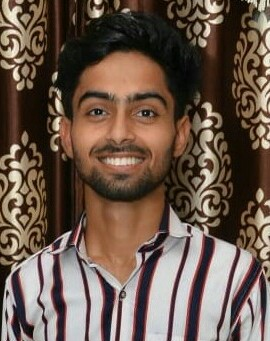
\includegraphics[height=3cm]{Sahil.jpeg}
        \end{flushright}
        
\end{multicols}


% Education
\section{\underline{Education}}

    \subsection{\textbf{Bachelor of Technology (B.Tech), Computer Science \& Engineering}\newline 
    \textmd{Manipal Institute of Technology, Manipal --  2018 - 2022 -- CGPA: 8.30/10}}
    
    \subsection{\textbf{Senior Secondary (XII), Science}\newline 
    \textmd{ Shiksha Niketan Higher Secondary, Jammu -- Year of completion: 2018 --  Percentage: 93.00\%}}
    
    % \subsection{\textbf{Secondary (X),Science}\newline 
    % \textmd{Fatima Covent, Jammu -- Year of completion: 2016 -- Percentage: 90.20\%}}
   
\section{\underline{Internship}}

    \subsection{\textbf{Backend Engineer}
    \textmd{- FOLK Developers (Ongoing)}\newline 
    \textmd{Working on Backend Development with Python and Google Cloud Platform. Working with Google Firebase tools like Firestore database , Cloud Functions etc. } }
    
\section{\underline{Projects}}

    \subsection{\textbf{Finland Labs and IIT Roorkee - ML \& AI Using Covid 19 Virus Data Analysis Workshop:}
    \textmd{Applied Data Pre-processing, Visualization and Machine Learning techniques to make the predictions how the cases will increase/decrease in the country. } }

    \subsection{\textbf{Web Scrapper:}
    \textmd{Developed a Web Scrapper using Python APIs to scrape the reviews of a product from some commercial website.
    Stored that in data using MongoDB and then displayed it using front-end frameworks.}}

    \subsection{\textbf{Boston Housing Price Prediction:}
    \textmd{Applied Data Prepossessing,Data Visualization and Machine Learning techniques to create a 
    Linear Regression model to predict the house prices in Boston,Massachusetts. } }

    % \subsection{\textbf{Data Exchange in Heterogeneous Systems( Collaborative project )- ongoing:}
    % \textmd{The objective of this project is to experience the real
    % world problem of data exchange in a automatic fashion between different generations 
    % of applications.So we are trying to prove $sin^2(x) + cos^2(x)=1$ } 
    % % \begin{equation}
    % %     sin^2(x) + cos^2(x)=1
    % % \end{equation} 
    % \textmd{Here we consider three systems communicating the data.}
    % }

    \subsection{\textbf{Routing System(Collaborative project )}
    \textmd{The objective of this project is to track the user and to display the route between two mentioned locations spread across karnataka. Done using Python, JavaScript and some HTML. } 
    % \begin{equation}
    %     sin^2(x) + cos^2(x)=1
    % \end{equation} 
    }
 % Courses
\section{\underline{Courses}}


    \subsection{\textbf{Machine Learning using Python Online-Project-based-course }
    \textmd{- Skyfi Labs}}

    \subsection{\textbf{Data Analysis and Data Visualization}
    \textmd{- Ineuron}}

    \subsection{\textbf{Python Programming}
    \textmd{- Ineuron}}
    
    \subsection{\textbf{Statistics for Data Science}
    \textmd{- Ineuron}}

    \subsection{\textbf{ML and AI using COVID-19 virus Data Analysis workshop}
    \textmd{- Finland Labs}}

    \subsection{\textbf{Accessing web Data using Python}
    \textmd{- Coursera}}

    \subsection{\textbf{Google Crash Course on Python}
    \textmd{- Coursera}}

    \subsection{\textbf{Python by University of Michigan}
    \textmd{- Coursera}}
    

 % Skills
 \section{\underline{Skills}}

    \subsection{\textbf{Programming Languages:}
    \textmd{Fluent in C/C++, Python }\newline
    \textmd{Familiar with : Java, SQL, Verilog, Fortran, {\LaTeX},Linux Shell Scripting, fair acquaintance
    with ARM assembly programming (NXP LPC 1768) } }

    \subsection{\textbf{Libraries and Frameworks:}\newline
    \textbf{Python:}\textmd{- Numpy, Pandas,Scikit-Learn,Matplotlib,seaborn and some others.}\newline
    \textbf{C++:}\textmd{- Standard Template Library(STL)}\newline
    \textbf{Java:}\textmd{- JavaFX GUI.}\newline
    \textbf{Web Development :}\textmd{- HTML, CSS , JavaScript, Bootstrap, JQuery and Django}\newline
    \textbf{IDEs used :}\textmd{- CodeBlocks, Sublime Text, PyCharm, Atom, Jupyter Notebook, Eclipse, Visual Studio Code and some others.}}
    \subsection{\textbf{Databases:}
    \textmd{Firestore, MySQL, NoSQL, MongoDB}}
    \subsection{\textbf{Others:}
    \textmd{Database Management Systems , Data Pre-processing and Data Analysis, Web Scrapping, REST API,}}


 % Skills


\section{\underline{Leadership/Involvement}}
    \subsection{\textmd{-Member of ACM college club. }\newline
    \textmd{-Member of College and university Athletics team. }\newline
    \textmd{-Member of Organising team of the Manipal Marathon. }\newline
    \textmd{-Interviewed second year students for ACM club recruitment. }\newline
    \textmd{-Awarded with Best Athlete Award in Revels'19, the National Cultural and Sports Fest of MIT. Won many other medals in Athletics. }\newline
    \textmd{-Part time tutor for Secondary students. }\newline
    \textmd{-PMSSS, AICTE scholarship holder for graduation.}}

%     Languages
% \section{\underline{Languages}}

%     \subsection{\textbf{English, Hindi, Punjabi, Dogri}}

% \end{document}
\end{document}
